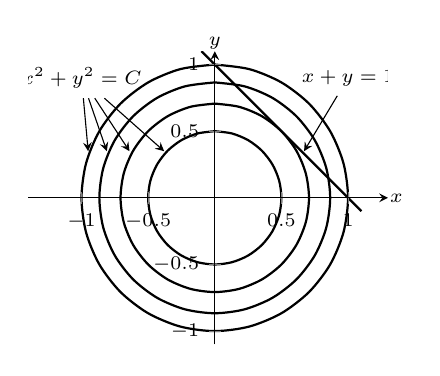
\begin{tikzpicture}[>=stealth]
\begin{axis}%
[width=175pt,tick label style={font=\scriptsize},axis on top,
			axis lines=center,
			axis equal,
			%view={135}{20},
			name=myplot,
			%xtick=\empty,
			%ytick={5},
			ztick=\empty,
			minor xtick=1,
			xtick = {-1,-.5,...,1},
			minor ytick=1,
			ymin=-1.1,ymax=1.1,
			xmin=-1.2,xmax=1.1,
			%zmin=-.5, zmax=1.1,
			every axis x label/.style={at={(axis cs:\pgfkeysvalueof{/pgfplots/xmax},0,0)},xshift=3pt,yshift=0pt},
				xlabel={\scriptsize $x$},
			every axis y label/.style={at={(axis cs:0,\pgfkeysvalueof{/pgfplots/ymax},0)},xshift=0pt,yshift=3pt},
				ylabel={\scriptsize $y$},
			%every axis z label/.style={at={(axis cs:0,0,\pgfkeysvalueof{/pgfplots/zmax})},xshift=0pt,yshift=4pt},
				%zlabel={\scriptsize $z$},
			]

%\addplot3[domain=-1:1,,y domain=-1:1,surf,%fill=white,
%colormap={mp2}{rgb=(.7,.7,1); rgb=(.9,.9,1)},
%faceted color=black!40,samples=25,samples y=25,very thin,z buffer=sort] {1- x^2 - y^2};

%\addplot3[domain=-1:1,,y domain=-1:1,surf,%fill=white,
%colormap={mp2}{\colormapplaneone},
%samples=25,samples y=25, z buffer=sort,%shader=interp,opacity=.75
%] {1- x^2 - y^2};

%\addplot3 [thick,{\colortwo}, smooth,domain=-0:1,samples=10,samples y=0] ({x},{1-x},{1 - x^2 - (1-x)^2});
\addplot [thick,{\colortwo}, smooth,domain=-.1:1.1,samples=2,samples y=0] ({x},{1-x});

\addplot[thick,{\colorone},smooth,domain=0:2*pi,samples=25,samples y=0]({1*sin(deg(x))},{1*cos(deg(x))});
\addplot[thick,{\colorone},smooth,domain=0:2*pi,samples=25,samples y=0]({.866*sin(deg(x))},{.866*cos(deg(x))});
\addplot[thick,{\colorone},smooth,domain=0:2*pi,samples=25,samples y=0]({.7071*sin(deg(x))},{.7071*cos(deg(x))});
\addplot[thick,{\colorone},smooth,domain=0:2*pi,samples=25,samples y=0]({.5*sin(deg(x))},{.5*cos(deg(x))});

\draw node at (axis cs:-1,.9) (a) {\scriptsize $x^2 + y^2 = C$};
\draw [black,->] (a)--(axis cs:-.81,.35);
\draw [black,->] (a)--(axis cs:-.64,.35);
\draw [black,->] (a)--(axis cs:-.95,.35);
\draw [black,->] (a)--(axis cs:-.38,.35);

\draw node at (axis cs:1,.9) (b) {\scriptsize $x + y = 1$};
\draw [black,->] (b)--(axis cs:.67,.35);

%\addplot3 [thick,{\colortwo}, smooth,domain=0:2,samples=10,samples y=0] ({x},{-1.5*x+1},{x^2-(-1.5*x+1)^2+5});
%\addplot3 [thick,{\colortwo}, smooth,domain=-1:2,samples=10,samples y=0] ({x},{-2},{x^2-4+5});
%
%\addplot3 [thick,{\colortwo}, smooth,dashed,domain=-1:0,samples=10,samples y=0] ({x},{3*x+1},{0});
%\addplot3 [thick,{\colortwo}, smooth,dashed,domain=0:2,samples=10,samples y=0] ({x},{-1.5*x+1},{0});
%\addplot3 [thick,{\colortwo}, smooth,dashed,domain=-1:2,samples=10,samples y=0] ({x},{-2},{0});


%\filldraw [black,] (axis cs:.5,.5,.5) circle (1pt);
%\filldraw [black,] (axis cs:-1,-2,2) circle (1pt);
%\filldraw [black,] (axis cs:-.375,-0.125,5.125) circle (1pt);
%\filldraw [black,] (axis cs:0,-2,1) circle (1pt);
%\filldraw [black,] (axis cs:2,-2,5) circle (1pt);
%\filldraw [black,] (axis cs:0,1,4) circle (1pt);
%\filldraw [black,] (axis cs:1.2,-0.8,5.8) circle (1pt);


\end{axis}


\end{tikzpicture}












